\section{Baryons and color}
\label{sec:baryons-color}

% ============================================================
\subsection{Baryon wavefunction and the antisymmetry problem}
\label{subsec:baryon-antisymmetry}

Baryons are bound states of three quarks, and since quarks are spin-$\tfrac{1}{2}$
fermions the Pauli principle requires the total wavefunction to be antisymmetric
under the exchange of any pair of constituents. In the non-relativistic quark model
the wavefunction factorizes into a flavor part, a spin part and a spatial part,
\begin{equation}
    \psi = \Phi_{\text{flavor}}\,\chi_{\text{spin}}\,R(\vec{r}),
    \label{eq:baryon-Psi-nocolor}
\end{equation}
which is the form available before color is introduced \cite[Ch.~13]{Amsler2018}.
The spatial factor of the ground-state baryons carries no orbital angular momentum,
$L = 0$, and is therefore symmetric, so the required antisymmetry has to be supplied
by the combined flavor and spin factors alone.

The building blocks are fixed by the group-theoretical decompositions of three
fundamental representations. For flavor one finds
\begin{equation}
    \mathbf{3} \otimes \mathbf{3} \otimes \mathbf{3}
    = \mathbf{10}_{S} \oplus \mathbf{8}_{MS} \oplus \mathbf{8}_{MA}
      \oplus \mathbf{1}_{A},
    \label{eq:flavor-3x3x3}
\end{equation}
giving a totally symmetric decuplet, two octets of mixed symmetry and a totally
antisymmetric singlet \cite[Ch.~13]{Amsler2018}. For the three quark spins the
analogous coupling reads
\begin{equation}
    \mathbf{2} \otimes \mathbf{2} \otimes \mathbf{2}
    = \mathbf{4}_{S} \oplus \mathbf{2}_{MS} \oplus \mathbf{2}_{MA},
    \label{eq:spin-2x2x2}
\end{equation}
that is, one fully symmetric spin-$\tfrac{3}{2}$ quadruplet and two spin-$\tfrac{1}{2}$
doublets of mixed symmetry. Note that no totally antisymmetric combination of three
spin-$\tfrac{1}{2}$ states exists, a fact that will prove decisive below.

Experimentally the baryons of lowest mass arrange themselves into exactly the
multiplets that these representations predict: a spin-$\tfrac{1}{2}$ octet containing
the proton and the neutron, and a spin-$\tfrac{3}{2}$ decuplet containing the
$\Delta(1232)$. Both are observed as the ground states, with $L = 0$ and hence a
symmetric spatial wavefunction \cite[Ch.~13]{Amsler2018}.

The difficulty becomes most transparent at the corners of the decuplet, where the
three quark flavors are identical. The state
\begin{equation}
    \Delta^{++} = \ket{uuu}\,\ket{\uparrow\uparrow\uparrow}\,\ket{L=0}
\end{equation}
is symmetric in flavor, symmetric in spin and symmetric in space, so the product
\eqref{eq:baryon-Psi-nocolor} is \emph{totally symmetric} under quark exchange. The
same holds for the $\Delta^-(ddd)$ and the $\Omega^-(sss)$. Such configurations
manifestly violate the Pauli principle for identical fermions, and with only the
factors in \eqref{eq:baryon-Psi-nocolor} at hand there is no way to repair the
symmetry \cite[Ch.~10]{Amsler2018}. The quark model, otherwise so successful in
accounting for the observed multiplets, is thereby driven into a genuine
contradiction whose resolution requires an additional degree of freedom.

\begin{figure}[htbp]
  \centering
  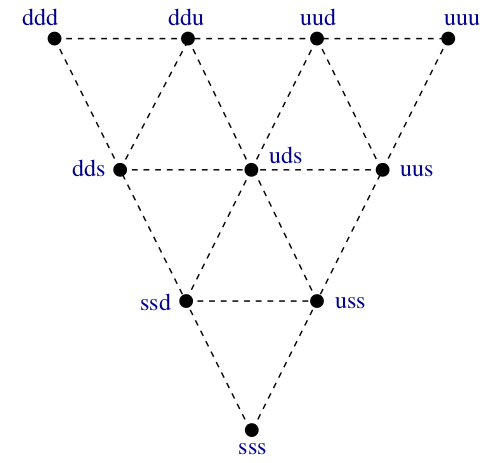
\includegraphics[width=0.55\textwidth]{Figures/decuplet_corners.png}
  \caption{Weight diagram of the spin-$\tfrac{3}{2}$ baryon decuplet. The three
  corner states $\Delta^{++}(uuu)$, $\Delta^-(ddd)$ and $\Omega^-(sss)$ are built
  from three identical quarks with aligned spins and a symmetric $L=0$ spatial
  wavefunction, and are therefore totally symmetric under exchange. Adapted
  from the lecture slides (week 19, "Baryons in SU(6)").}
  \label{fig:decuplet-corners}
\end{figure}

\FloatBarrier

% ============================================================
\subsection{Baryons in SU(6) and the ``56''-plet}
\label{subsec:su6-56plet}

The flavor and spin degrees of freedom can be combined into a single larger symmetry
by embedding the three flavors and the two spin states into a sixfold fundamental
representation. Coupling three such sextets and reducing the product with the help of
Young tableaux gives
\begin{equation}
    \mathbf{6} \otimes \mathbf{6} \otimes \mathbf{6}
    = \mathbf{56}_{S} \oplus \mathbf{70}_{MS} \oplus \mathbf{70}_{MA}
      \oplus \mathbf{20}_{A},
    \label{eq:su6-6x6x6}
\end{equation}
where the subscripts again record the permutation symmetry \cite[Ch.~13]{Amsler2018}.
Each $\mathrm{SU}(6)$ supermultiplet decomposes into definite combinations of an
$\mathrm{SU}(3)$ flavor multiplet and a definite total quark spin. The totally
symmetric $\mathbf{56}$ contains precisely the observed ground states,
\begin{equation}
    \mathbf{56} = (\mathbf{8},\, s=\tfrac{1}{2}) \;\oplus\; (\mathbf{10},\, s=\tfrac{3}{2}),
\end{equation}
that is, the spin-$\tfrac{1}{2}$ octet of nucleons and the spin-$\tfrac{3}{2}$
decuplet headed by the $\Delta(1232)$ \cite[Ch.~13]{Amsler2018}. The ground-state
baryons therefore fit the ``56''-plet without exception, which at first sight is a
remarkable success of the scheme.

The flavor wavefunctions that enter these assignments illustrate how the symmetry is
realized. For the $\Delta$ the totally symmetric flavor function is
\begin{equation}
    \Phi_{\Delta} = \sqrt{\tfrac{1}{3}}
    \big[\, uud + (ud + du)u \,\big],
\end{equation}
while the two mixed-symmetry partners needed for the octet read
\begin{equation}
    \Phi_{MA} = \sqrt{\tfrac{1}{2}}\,\big[\,(ud - du)u\,\big],
    \qquad
    \Phi_{MS} = \sqrt{\tfrac{1}{6}}\,\big[\,(ud + du)u - 2\,uud\,\big].
\end{equation}
A totally symmetric spin-$\tfrac{1}{2}$ wavefunction is then assembled from the
mixed-symmetric and mixed-antisymmetric flavor and spin factors, the proton being the
symmetric combination $\tfrac{1}{\sqrt{2}}\,(\Phi_{MS}\chi_{MS}
+ \Phi_{MA}\chi_{MA})$ \cite[Ch.~13]{Amsler2018}.

This is exactly where the antisymmetry problem of Sect.~\ref{subsec:baryon-antisymmetry}
returns in its sharpest form. The $\mathbf{56}$ is totally symmetric in the combined
flavor--spin variables, and for the ground states the orbital wavefunction $R(\vec r)$
with $L=0$ is symmetric as well. The product
\begin{equation}
    \Psi^{\text{total}} = \Phi_{\text{flavor}}\,\chi_{\text{spin}}\,R(\vec{r})
\end{equation}
is then symmetric, in direct conflict with the Pauli principle, which demands a
totally antisymmetric baryon. The very multiplet that accommodates all the observed
ground states is the one with the wrong overall symmetry, so the success of the
classification and its apparent failure under fermion statistics are two sides of the
same fact \cite[Ch.~13]{Amsler2018}.

\FloatBarrier

% ============================================================
\subsection{Magnetic moments and the constituent quark masses}
\label{subsec:magnetic-moments}

Before turning to color it is worth extracting a quantitative prediction from the
$\mathrm{SU}(6)$ wavefunctions just constructed. The magnetic moments of the ground-state
baryons are among the earliest and most convincing successes of the quark model, and they
provide the standard route to the \emph{constituent} quark masses---the effective masses a
quark acquires inside a hadron, much larger than the bare masses generated by the Higgs
mechanism.

Treating the quarks as point-like Dirac fermions with $g = 2$, each carries a magnetic
moment $\mu_i = Q_i e / 2 m_i$ aligned with its spin. The moment of a baryon is the
expectation value of the sum of the three quark moments in the state with maximal spin
projection,
\begin{equation}
    \mu_B = \frac{e}{2 m_q}
    \bra{B} \sum_{i=1}^{3} Q_i \,\sigma_{3}(i) \ket{B},
    \label{eq:magnetic-moment-operator}
\end{equation}
where $Q_i$ is the quark charge in units of $e$, $\sigma_3(i)$ acts on the spin of the
$i$-th quark, and $m_q = m_u = m_d$ in the isospin-symmetric limit
\cite[Ch.~15]{Amsler2018}.

\paragraph{Worked example: the neutron and the light constituent mass.}
The neutron is the $udd$ member of the octet, with the spin--flavor wavefunction obtained
from the proton one by $u \leftrightarrow d$. Written out for spin projection
$+\tfrac{1}{2}$, the totally symmetric combination gives, for each quark, a probability
$\tfrac{1}{3}$ of carrying spin antiparallel to the baryon and $\tfrac{2}{3}$ parallel,
weighted so that the expectation value of $\sigma_3$ is $-\tfrac{1}{3}$ for the two
like-flavor quarks and $+\tfrac{4}{3}$ for the odd one. Evaluating
Eq.~\eqref{eq:magnetic-moment-operator} on the octet wavefunctions gives, for the two
members of the nucleon doublet,
\begin{equation}
    \mu_p = \frac{4}{3}\,\mu_u - \frac{1}{3}\,\mu_d ,
    \qquad
    \mu_n = \frac{4}{3}\,\mu_d - \frac{1}{3}\,\mu_u ,
    \label{eq:mu-n-setup}
\end{equation}
the odd-flavor quark entering with weight $-\tfrac13$ and the like-flavor pair with
$+\tfrac43$. Inserting $\mu_u = \tfrac{2}{3}\,e/2m_q$ and $\mu_d = -\tfrac{1}{3}\,e/2m_q$,
\begin{equation}
    \mu_n = \left(-\frac{4}{9} - \frac{2}{9}\right)\frac{e}{2m_q}
          = -\,\frac{e}{3 m_q},
    \qquad
    \mu_p = \left(\frac{8}{9} + \frac{1}{9}\right)\frac{e}{2m_q}
          = +\,\frac{e}{2 m_q}.
    \label{eq:mu-n}
\end{equation}
The model therefore
predicts the ratio
\begin{equation}
    \frac{\mu_p}{\mu_n} = -\frac{3}{2},
    \label{eq:mu-ratio}
\end{equation}
against the measured $\mu_p/\mu_n = 2.793/(-1.913) = -1.46$---a parameter-free prediction accurate to a few percent, and
historically one of the strongest arguments that the quarks are real dynamical objects
rather than a bookkeeping device.

Equation~\eqref{eq:mu-n} can be read backwards. Inserting the measured neutron moment
$\mu_n = -1.913\,\mu_N$, with the nuclear magneton $\mu_N = e/2M_p$, gives
\begin{equation}
    m_q = \frac{2 M_p}{3 \times 1.913} \;\approx\; 327\;\mathrm{MeV},
    \label{eq:mq-from-mun}
\end{equation}
close to the value $m_u \simeq m_d \simeq 350\;\mathrm{MeV}$ usually quoted for the light
constituent masses. Amsler runs the same inversion through the \emph{proton} instead,
$\mu_p = 2.79\,\mu_N = e/2m$, obtaining $m = M_p/2.79 = 336\;\mathrm{MeV}$
\cite[Ch.~14]{Amsler2018}; the small difference between the two routes is a measure of how
far the model is from exact. The same calculation is carried out by Halzen and Martin
\cite[Ch.~2]{HalzenMartin1984} and by Perkins \cite[Ch.~4]{Perkins2000}.

\paragraph{Worked example: the strange quark mass from the $\Lambda$.}
The $\Lambda$ is especially clean. Its $ud$ pair is coupled to isospin $I=0$ and hence,
by the symmetry of the octet wavefunction, to spin $s=0$; the two light quarks therefore
contribute nothing to the moment, and the entire spin of the $\Lambda$ is carried by the
strange quark. Consequently
\begin{equation}
    \mu_\Lambda = \mu_s = \frac{Q_s e}{2 m_s} = -\,\frac{e}{6 m_s}.
    \label{eq:mu-lambda}
\end{equation}
With the measured $\mu_\Lambda = -0.613\,\mu_N$ this yields
\begin{equation}
    m_s = \frac{M_p}{3 \times 0.613} \;\approx\; 510\;\mathrm{MeV},
    \label{eq:ms-from-mulambda}
\end{equation}
in good agreement with the constituent value $m_s \simeq 500\;\mathrm{MeV}$. Amsler's
treatment of the hyperon moments proceeds identically, deducing the vanishing $ud$
contribution from $I(ud) = 0$ and hence $s(ud) = 0$ \cite[Ch.~14]{Amsler2018}. The difference
$m_s - m_q \approx 180\;\mathrm{MeV}$ is of the same order as the $130$--$150\;\mathrm{MeV}$
per unit of strangeness that governs the equal-spacing rule of Sect.~\ref{subsec:gmo}. Constituent masses obtained this
way are collected in Appendix~\ref{app:useful-tables}.

\FloatBarrier

% ============================================================
\subsection{Color as a new degree of freedom}
\label{subsec:color-dof}

The resolution, proposed in the mid-1960s by Greenberg and by Han and Nambu, and
developed by Gell-Mann, is to endow each quark flavor with a further internal quantum
number called \emph{color} \cite[Ch.~10]{Amsler2018}. Every quark comes in three
color states, labeled red ($r$), green ($g$) and blue ($b$), which span the
fundamental triplet of a new symmetry group $\mathrm{SU}(3)_{c}$. Unlike flavor
$\mathrm{SU}(3)$, which is badly broken by the quark mass differences, the color
symmetry $\mathrm{SU}(3)_{c}$ is taken to be exact.

The color states couple in the same way as the flavors,
\begin{equation}
    \mathbf{3} \otimes \mathbf{3} \otimes \mathbf{3}
    = \mathbf{10}_{S} \oplus \mathbf{8}_{MS} \oplus \mathbf{8}_{MA}
      \oplus \mathbf{1}_{A},
\end{equation}
and it is the totally antisymmetric singlet $\mathbf{1}_{A}$ that is used to restore
the overall antisymmetry of the baryon \cite[Ch.~10]{Amsler2018}. Explicitly, the
antisymmetric color wavefunction of three quarks is
\begin{equation}
\begin{split}
    \lambda_{\text{color}}(q_1 q_2 q_3) = \frac{1}{\sqrt{6}}
    \big[\, & q_1(r)q_2(g)q_3(b) + q_1(b)q_2(r)q_3(g) + q_1(g)q_2(b)q_3(r) \\
    & - q_1(g)q_2(r)q_3(b) - q_1(b)q_2(g)q_3(r) - q_1(r)q_2(b)q_3(g) \,\big].
\end{split}
\end{equation}
Multiplying the symmetric flavor--spin--space wavefunction of the ``56''-plet by this
antisymmetric color factor yields a total wavefunction
\begin{equation}
    \psi = \Phi_{\text{flavor}}\,\chi_{\text{spin}}\,\lambda_{\text{color}}\,R(\vec{r}),
    \label{eq:full-Psi-color}
\end{equation}
in which the symmetric product $\Phi_{\text{flavor}}\,\chi_{\text{spin}}\,R(\vec{r})$
is multiplied by the antisymmetric $\lambda_{\text{color}}$, so that the result is
antisymmetric and the Pauli principle is satisfied \cite[Ch.~10]{Amsler2018}. The
$\Delta^{++}$, $\Delta^-$ and $\Omega^-$ are thereby rescued precisely because their
color factor carries the antisymmetry that the rest of the wavefunction lacks.

A baryon built from the color singlet is colorless, or ``white''. This is the
quantitative content of the observation that all hadrons seen in nature are color
singlets: color charge itself is never observed in isolation, and only color-neutral
combinations propagate as free particles \cite[Ch.~10]{Amsler2018}. The exactness of
$\mathrm{SU}(3)_{c}$ together with this confinement of color provides the foundation on which Quantum Chromodynamics is built.

\FloatBarrier

% ============================================================
\subsection{Gluons and the color octet}
\label{subsec:gluons-octet}

If color is to be a dynamical charge, the force between quarks must transmit it. The
mediators of the strong interaction, the gluons, therefore carry one unit of color and
one unit of anticolor, color being conserved at each quark--gluon vertex
\cite[Ch.~10]{Amsler2018}. The nine combinations of a color with an anticolor reduce
in the same manner as the $q\bar q$ mesons,
\begin{equation}
    \mathbf{3} \otimes \overline{\mathbf{3}} = \mathbf{1} \oplus \mathbf{8},
\end{equation}
splitting the color--anticolor states into a singlet and an octet. The eight octet
states,
\begin{equation}
    r\bar g,\; r\bar b,\; g\bar r,\; g\bar b,\; b\bar r,\; b\bar g,\;
    \tfrac{1}{\sqrt{2}}(r\bar r - g\bar g),\;
    \tfrac{1}{\sqrt{6}}(r\bar r + g\bar g - 2 b\bar b),
\end{equation}
are the eight physical gluons, the gauge fields of QCD, while the remaining colorless
combination is the singlet
\begin{equation}
    \tfrac{1}{\sqrt{3}}\,(r\bar r + g\bar g + b\bar b).
\end{equation}

The singlet gluon is not realized in nature, and confinement provides the reason. A
color-singlet gluon would itself be colorless, and a colorless mediator could be
emitted as a free particle and exchanged between two color-singlet hadrons, giving rise
to a long-range strong force with strong coupling \cite[Ch.~10]{Amsler2018}. No such
force is observed, so the singlet does not appear as a physical field and exactly eight
colored gluons remain. Because the gluons carry color themselves, they interact with one
another, a non-Abelian feature that distinguishes QCD from electrodynamics and underlies
both confinement and asymptotic freedom.

\FloatBarrier

% ============================================================
\subsection{Baryon supermultiplets and excited states}
\label{subsec:supermultiplets}

With the total wavefunction antisymmetrized by color as in \eqref{eq:full-Psi-color},
the requirement of antisymmetry can be reformulated for the visible degrees of freedom:
since $\lambda_{\text{color}}$ is always the antisymmetric singlet, the remaining product
$\Phi_{\text{flavor}}\,\chi_{\text{spin}}\,R(\vec{r})$ must be totally
\emph{symmetric}. For the ground states the orbital factor is symmetric and this selects
the ``56''-plet. The excited baryons, however, may carry orbital angular momentum, which
opens additional possibilities for the spatial wavefunction $R(\vec{r})$ and hence for the
$\mathrm{SU}(6)$ content \cite[Ch.~15]{Amsler2018}.

The internal motion of three quarks is conveniently described by the two Jacobi
coordinates
\begin{equation}
    \vec{\rho} = \tfrac{1}{\sqrt{2}}\,(\vec{x}_1 - \vec{x}_2),
    \qquad
    \vec{\lambda} = \tfrac{1}{\sqrt{6}}\,(\vec{x}_1 + \vec{x}_2 - 2\,\vec{x}_3),
\end{equation}
where $\vec{\rho}$ describes the relative motion within a quark pair and $\vec{\lambda}$
the motion of the third quark relative to that pair. The associated orbital angular
momenta determine the parity,
\begin{equation}
    P(qqq) = (-1)^{L_{\rho}}\,(-1)^{L_{\lambda}},
\end{equation}
so that ground-state baryons with $L_{\rho} = L_{\lambda} = 0$ have $J^P =
\tfrac{1}{2}^+$ or $\tfrac{3}{2}^+$ \cite[Ch.~13]{Amsler2018}. In the harmonic-oscillator
model the excitations are organized by the band number
\begin{equation}
    N = 2n + L = 2 n_\rho + 2 n_\lambda + L_{\rho} + L_{\lambda},
\end{equation}
and the spectrum is classified under the combined $\mathrm{SU}(6) \times O(3)$ symmetry,
each level being labeled by an $\mathrm{SU}(6)$ multiplet and its orbital angular momentum $L$ \cite[Ch.~15]{Amsler2018}.

The mixed-symmetry and antisymmetric $\mathrm{SU}(6)$ multiplets, which cannot describe
the symmetric ground states, become accessible once the orbital wavefunction itself
carries a definite mixed or antisymmetric character. The $\vec{\rho}$ excitation is
antisymmetric and the $\vec{\lambda}$ excitation symmetric under exchange of the first two
quarks, and combining these with mixed flavor--spin functions produces a totally symmetric
product. In this way the $\mathbf{70}$-plet appears as the lowest negative-parity band
($N=1$, $L=1$), decomposing into a spin-$\tfrac{3}{2}$ octet together with a decuplet, an
octet and a singlet of spin $\tfrac{1}{2}$, while the totally antisymmetric flavor singlet
$\Phi_A$, which has no place among the ground states, is realized only in these excited
multiplets, namely in the $\mathbf{70}$ and the $\mathbf{20}$
\cite[Ch.~15]{Amsler2018}. The $\mathrm{SU}(6)$ supermultiplets thus organize as
\begin{align}
    \mathbf{56}: &\quad s=\tfrac{1}{2}\ \text{octet},\;\; s=\tfrac{3}{2}\ \text{decuplet}, \nonumber\\
    \mathbf{70}: &\quad s=\tfrac{1}{2}\ \text{decuplet},\;\; s=\tfrac{3}{2}\ \text{octet},\;\;
                   s=\tfrac{1}{2}\ \text{octet},\;\; s=\tfrac{1}{2}\ \text{singlet}, \\
    \mathbf{20}: &\quad s=\tfrac{3}{2}\ \text{singlet},\;\; s=\tfrac{1}{2}\ \text{octet}. \nonumber
\end{align}

These predicted supermultiplets map onto the experimentally established excited baryons.
The known $N^{*}$ and $\Delta^{*}$ resonances, as well as the strange $\Lambda^{*}$ and
$\Sigma^{*}$ states, populate the bands expected from $\mathrm{SU}(6)\times O(3)$, with the
ground-state nucleons and $\Delta(1232)$ in the $(\mathbf{56},0^{+})$ at $N=0$ and the
lowest orbital excitations in the $(\mathbf{70},1^{-})$ at $N=1$
\cite[Ch.~15]{Amsler2018}. The model predicts many more excitations than have been seen;
several states couple only weakly to the pion--nucleon and kaon--nucleon channels used to
produce them, and no firmly established candidate has yet been assigned to the
$\mathbf{20}$-plet \cite[Ch.~15]{Amsler2018}.

The flavor content of the $\mathbf{20}$ has a striking consequence. A totally
\emph{antisymmetric} spatial wavefunction must be paired with the totally antisymmetric
flavor--spin multiplet, which is the $\mathbf{20}$, and the $\mathbf{20}$ contains only a
spin-$\tfrac12$ octet and a spin-$\tfrac32$ singlet---\emph{no decuplet}. Since the
$\Delta$ states live exclusively in flavor decuplets, it follows that a baryon with an
antisymmetric spatial wavefunction can exist as an $N^{*}$ (or $\Lambda^{*}$,
$\Sigma^{*}$, $\Xi^{*}$) but never as a $\Delta^{*}$. This is a clean, falsifiable
prediction of the scheme, and it is part of why the $\mathbf{20}$-plet remains so hard to
identify experimentally: the states it predicts are precisely those that couple most
weakly to the formation channels used to search for them \cite[Ch.~15]{Amsler2018}.

The lowest negative-parity band is the one most thoroughly explored. Combining $L=1$ with
the two spin values available in the $\mathbf{70}$ generates exactly five nucleon states
and two $\Delta$ states, listed in Table~\ref{tab:70-1minus}. The counting follows from
angular-momentum addition alone: for $s=\tfrac12$, $L\otimes s$ gives $J=\tfrac12,
\tfrac32$; for $s=\tfrac32$ it gives $J=\tfrac12,\tfrac32,\tfrac52$; and all carry
$P=-1$. The $\Delta$ sector is restricted to $s=\tfrac12$, because its flavor decuplet is
symmetric and must therefore pair with a mixed-symmetry spin function, so only two
$\Delta^{*}$ states appear.

\begin{table}[htbp]
    \centering
    \caption{The five $N^{*}$ and two $\Delta^{*}$ states of the
    $(\mathbf{70},1^{-})$ band at $N=1$, with their physical assignments.}
    \label{tab:70-1minus}
    \begin{tabular}{llll}
        \hline
        Flavor multiplet & Quark spin $s$ & $J^{P}$ & State \\
        \hline
        octet    & $\tfrac12$ & $\tfrac12^{-}$ & $N(1535)$ \\
        octet    & $\tfrac12$ & $\tfrac32^{-}$ & $N(1520)$ \\
        octet    & $\tfrac32$ & $\tfrac12^{-}$ & $N(1650)$ \\
        octet    & $\tfrac32$ & $\tfrac32^{-}$ & $N(1700)$ \\
        octet    & $\tfrac32$ & $\tfrac52^{-}$ & $N(1675)$ \\
        decuplet & $\tfrac12$ & $\tfrac12^{-}$ & $\Delta(1620)$ \\
        decuplet & $\tfrac12$ & $\tfrac32^{-}$ & $\Delta(1700)$ \\
        \hline
    \end{tabular}
\end{table}

Radial excitations follow the same band-number bookkeeping. Setting $L=0$ but
$n_{\rho}+n_{\lambda}=1$ gives $N=2$ with \emph{positive} parity, since
$P=(-1)^{L_{\rho}+L_{\lambda}}$ depends only on the orbital angular momenta and not on the
radial quantum numbers. A radial excitation therefore carries the same $J^{P}$ as the
state it excites: the first radial excitation of the nucleon is the Roper resonance
$N(1440)\tfrac12^{+}$, and that of the $\Delta(1232)$ is the $\Delta(1600)\tfrac32^{+}$.
The Roper's anomalously low mass---below the negative-parity $N(1535)$, contrary to the
naive oscillator ordering---is a long-standing puzzle discussed in
Sect.~\ref{subsec:transition-ff}. The band structure and the assignments of this section
follow Amsler's treatment of the light baryon excitations \cite[Ch.~15]{Amsler2018}.

\begin{figure}[htbp]
  \centering
  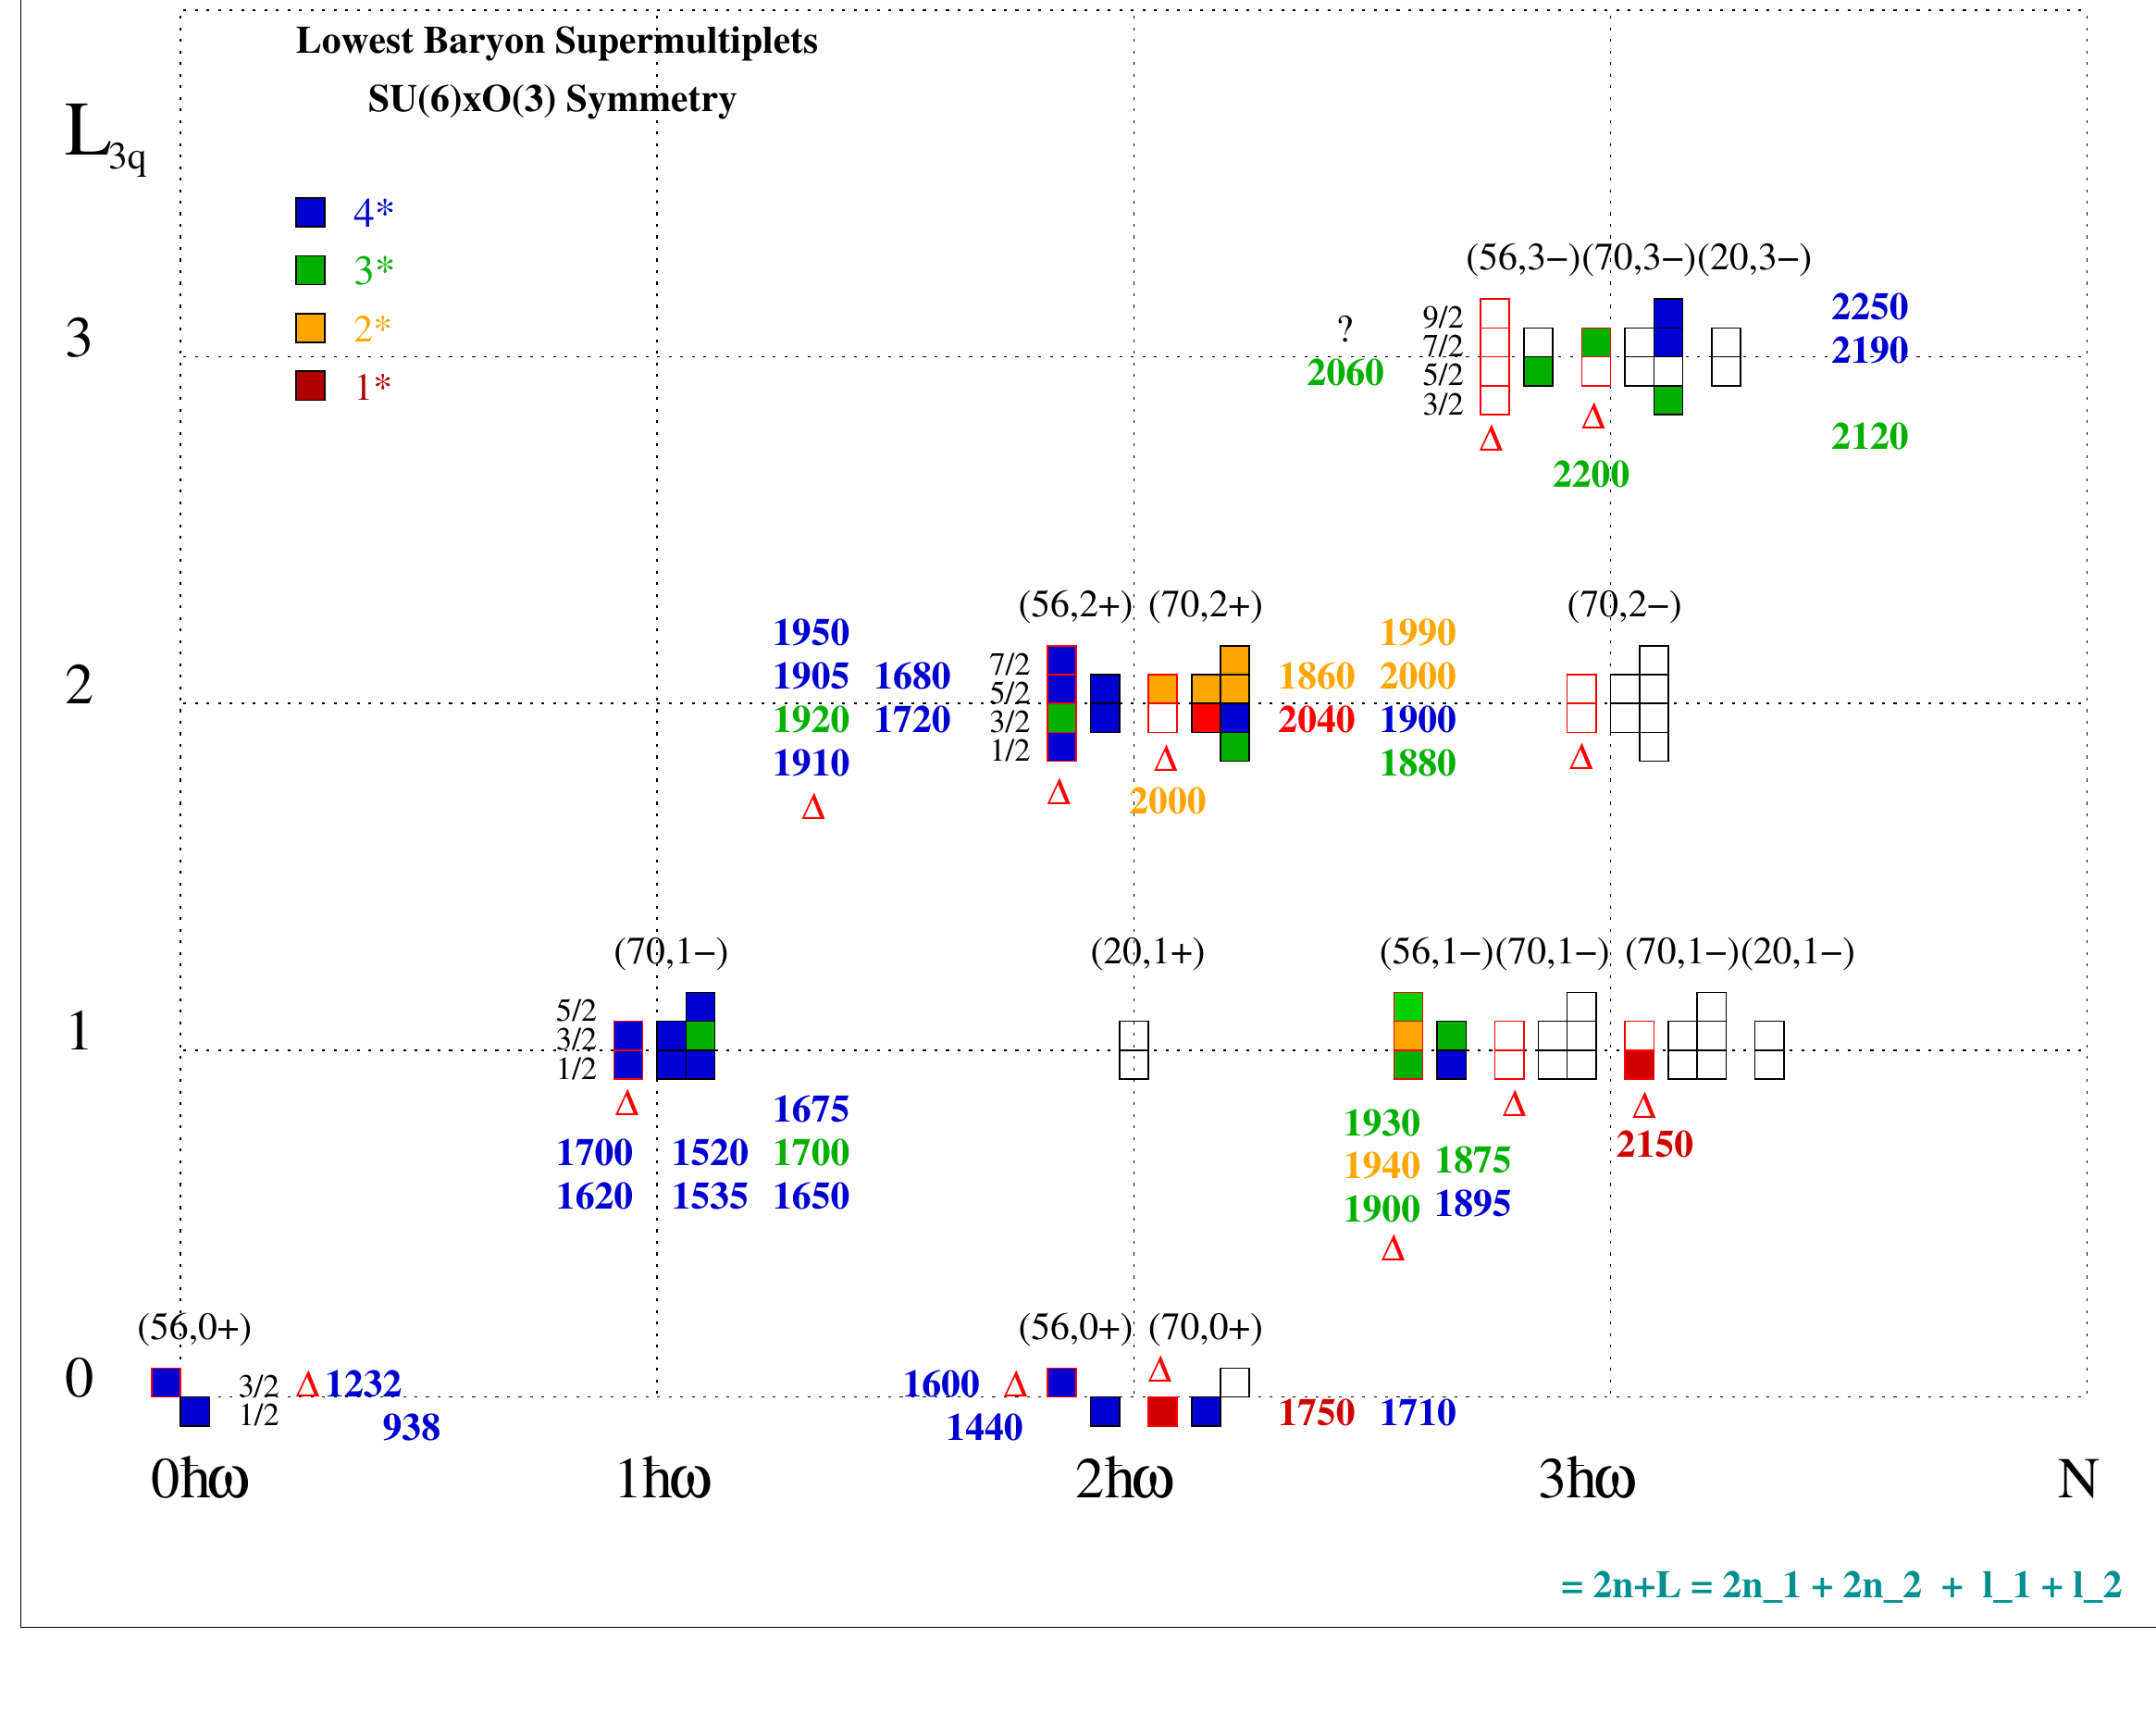
\includegraphics[width=0.9\textwidth]{Figures/baryon_supermultiplets.png}
  \caption{Distribution of the lowest baryon supermultiplets in the
  $\mathrm{SU}(6)\times O(3)$ harmonic-oscillator model as a function of orbital
  angular momentum $L$ and band number $N = 2n + L$, with the established
  $N^{*}$ and $\Delta^{*}$ assignments. Adapted from the lecture slides
  (week 20, "Multiplets $\leftrightarrow$ known $N^*$, $\Delta^*$-states").}
  \label{fig:baryon-supermultiplets}
\end{figure}

\FloatBarrier

% ============================================================
\subsection{Finding color in experiments}
\label{subsec:color-experiment}

Color was introduced to save the quark model, but its threefold character is not a
bookkeeping device: it can be measured. The cleanest counting experiment is the
annihilation of electron--positron pairs into hadrons through a virtual photon. Since the
photon couples to the quark electric charge, the total annihilation cross section into a
quark--antiquark pair of charge $e_f$ is, summing over all kinematically accessible final
states,
\begin{equation}
    \sigma_{\text{tot}}(e^+e^- \to f\bar f)
    \;\propto\; \sum_{\text{all } f\bar f \text{ pairs}} \frac{4\pi e_f^{2}}{3s},
\end{equation}
where $\sqrt{s}$ is the center-of-mass energy \cite[Ch.~10]{Amsler2018}. Normalizing the
hadronic cross section to that for muon pairs removes the common kinematic factors and
isolates the charge and color content,
\begin{equation}
    R = \frac{\sigma_{\text{tot}}(e^+e^- \to q\bar q)}
             {\sigma_{\text{tot}}(e^+e^- \to \mu^+\mu^-)}
      = N_{C} \sum_q e_q^{2},
    \label{eq:R-ratio}
\end{equation}
the factor $N_{C}$ arising because each quark flavor is produced in $N_{C}$ distinguishable
colors \cite[Ch.~10]{Amsler2018}.

The predictive power of \eqref{eq:R-ratio} lies in its step structure. As the energy
crosses the threshold for producing a new flavor, the ratio increases by $e_q^{2} N_{C}$.
Taking $N_{C} = 3$ one predicts $R = 2$ in the region where only the $u$, $d$ and $s$ quarks
are produced, rising to $R = 10/3$ above the charm threshold and to $R = 11/3$ once the
bottom quark contributes,
\begin{align}
    u,d:   &\quad \big(\tfrac{2}{3}\big)^2 + \big(\tfrac{1}{3}\big)^2 = \tfrac{5}{9}
            \;\Rightarrow\; \tfrac{5}{9}\,N_{C}, \nonumber\\
    u,d,s: &\quad \big(\tfrac{2}{3}\big)^2 + 2\big(\tfrac{1}{3}\big)^2 = \tfrac{2}{3}
            \;\Rightarrow\; \tfrac{2}{3}\,N_{C}\;(=2\ \text{for}\ N_{C}=3), \\
    u,d,s,c:   &\quad \;\Rightarrow\; \tfrac{10}{9}\,N_{C}, \nonumber\\
    u,d,s,c,b: &\quad \;\Rightarrow\; \tfrac{11}{9}\,N_{C}. \nonumber
\end{align}
The measured value of $R$ in the continuum between the resonances matches these
predictions only for $N_{C} = 3$, which is the central experimental statement that there are
three colors \cite[Ch.~10]{Amsler2018}. Figure~\ref{fig:R-ratio-steps} shows the
leading-order prediction with its characteristic increases at the open-flavor thresholds.

\begin{figure}[htbp]
    \centering
    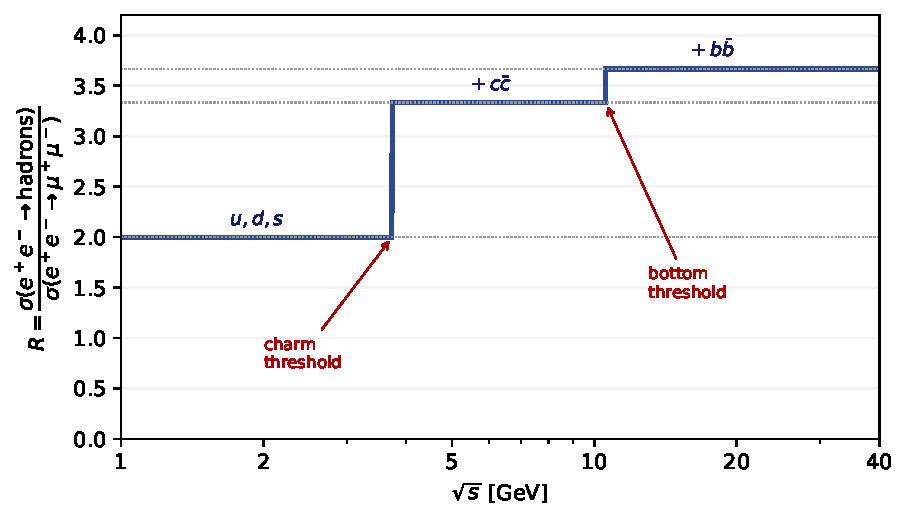
\includegraphics[width=0.7\textwidth]{Figures/R_ratio_steps.pdf}
    \caption{Leading-order prediction for the ratio $R = \sigma(e^+e^- \to
    \text{hadrons})/\sigma(e^+e^- \to \mu^+\mu^-) = N_{C} \sum_q e_q^2$ as a function of
    $\sqrt{s}$, for $N_{C} = 3$. The ratio increases by $e_q^2 N_{C}$ each time the energy
    crosses the threshold for producing a new quark flavor, giving $R = 2$ ($u,d,s$),
    $R = 10/3$ (adding $c$) and $R = 11/3$ (adding $b$). The smooth resonances are omitted.}
    \label{fig:R-ratio-steps}
\end{figure}

\begin{figure}[htbp]
  \centering
  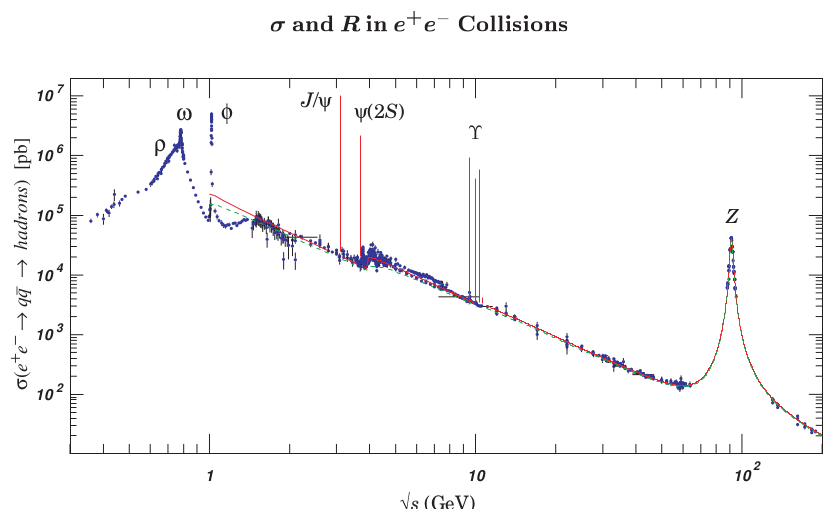
\includegraphics[width=0.9\textwidth]{Figures/R_measured_PDG.png}
  \caption{Measured cross section $\sigma(e^+e^-\to\mathrm{hadrons})$ (closely
  tracking the ratio $R$) over the full $\sqrt{s}$ range, showing the
  $\rho/\omega/\phi$ region, the narrow $J/\psi$ and $\psi(2S)$, the
  $\Upsilon$ states and the $Z$ pole. The smooth continuum between resonances
  sits on the plateaux predicted by $R = N_{C}\sum_q e_q^2$, requiring $N_{C}=3$.
  PDG compilation, adapted from the lecture slides (week 20, "Color -
  Experimental evidence for $N_C = 3$").}
  \label{fig:R-measured}
\end{figure}

The same factor of three appears in two further measurements. The decay $\pi^0 \to 2\gamma$
proceeds through a quark triangle whose amplitude is enhanced by the color sum, so that the
partial width scales as $N_{C}^{2}$ and the predicted rate agrees with experiment only for
three colors; without color the neutral-pion lifetime would be about nine times longer.
Likewise, the hadronic branching ratio of the $W^{+}$ boson, close to $66\%$, carries a
factor of three for each available quark color in the $u\bar d$ and $c\bar s$ channels
\cite[Ch.~10]{Amsler2018}. Taken together, the $e^+e^-$ ratio, the $\pi^0$ lifetime and the
$W$ branching fractions all point to the same conclusion, $N_{C} = 3$, which is the
experimental basis of QCD.

A related experimental fact, the strong suppression of flavor-changing neutral currents
such as $K^{+} \to \pi^{+}\nu\bar\nu$, is accounted for by the GIM mechanism and the
Cabibbo theory and was historically tied to the prediction of the charm quark, whose
$c\bar c$ bound states first appeared as the narrow $J/\psi$ resonance discussed in the
following section.

\FloatBarrier